\chapter{Conclusion}

The development of this report illustrates the ease of which a full-stack web application can be developed from the ground up using best industry standards. Being able to create a highly available, fault-resistant service is crucial for businesses trying to serve a SaaS or likewise application to their users. The security policies that can be enabled easily within AWS as well as how easy it is to create a robust fault-tolerant infrastructure from within AWS makes it ideal.
In summary, we believe that the project went very well with a few improvements we wish we could make, see Chapter~\ref{ch:future-enhancements}, however within the limitations we had we were able to implement everything we wanted to.

If we were to do this again, we would strive to be more aware of how much the infrastructure is costing during development, as almost half of the \$100 budget was used during this initial development, without any real users.

During development, we must also be more careful to ensure our IDE's are able to check spelling and evaluate our code before we make changes, as our group had spent hours on this trivial bug (Figure~\ref{fig:bug-fudge}) during the setup of RDS:
\begin{figure}[!htbp]
    \centering
    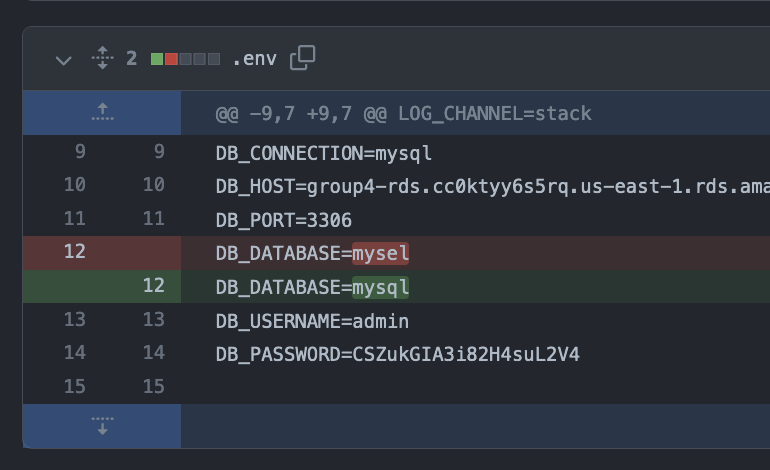
\includegraphics[width=\textwidth]{resources/rds/mysql.png}
    \caption{Major Bug Fixes Can be Small}
    \label{fig:bug-fudge}
\end{figure}